\section{Провисання дроту}

	Очевидно, що зі зміщенням дроту з центру трубки електричне поле також викривлюється(див. Рис.\ref{fig:elFieldCentered},\ref{fig:elField1mmShifted}) і траєкторії дрейфу електронів та іонів в трубці відповідно також змінюються (див. Рис.\ref{fig:electron_ion_track_sag}). Як наслідок змінюється залежність часу дрейфу від позиції треку в трубці(TR-відношення). Так що TR-відношення втрачає свою попередню симетрію. 
	
%	Easy to predict that the displacement of the wire invokes distorting an electric field(see figs~\ref{fig:elFieldCentered},\ref{fig:elField1mmShifted}) and drift path for electrons/ions inside the tube(see fig.\ref{fig:electron_ion_track} and fig.\ref{fig:electron_ion_track_sag}). The rt-relation for track reconstruction directly depend on the wire position in the tube. So rt-relation lose it's previous symmetry(see next sections).
	
	\begin{figure}[h!]
		\centering
		\subfloat[дріт строго по центру трубки]{
			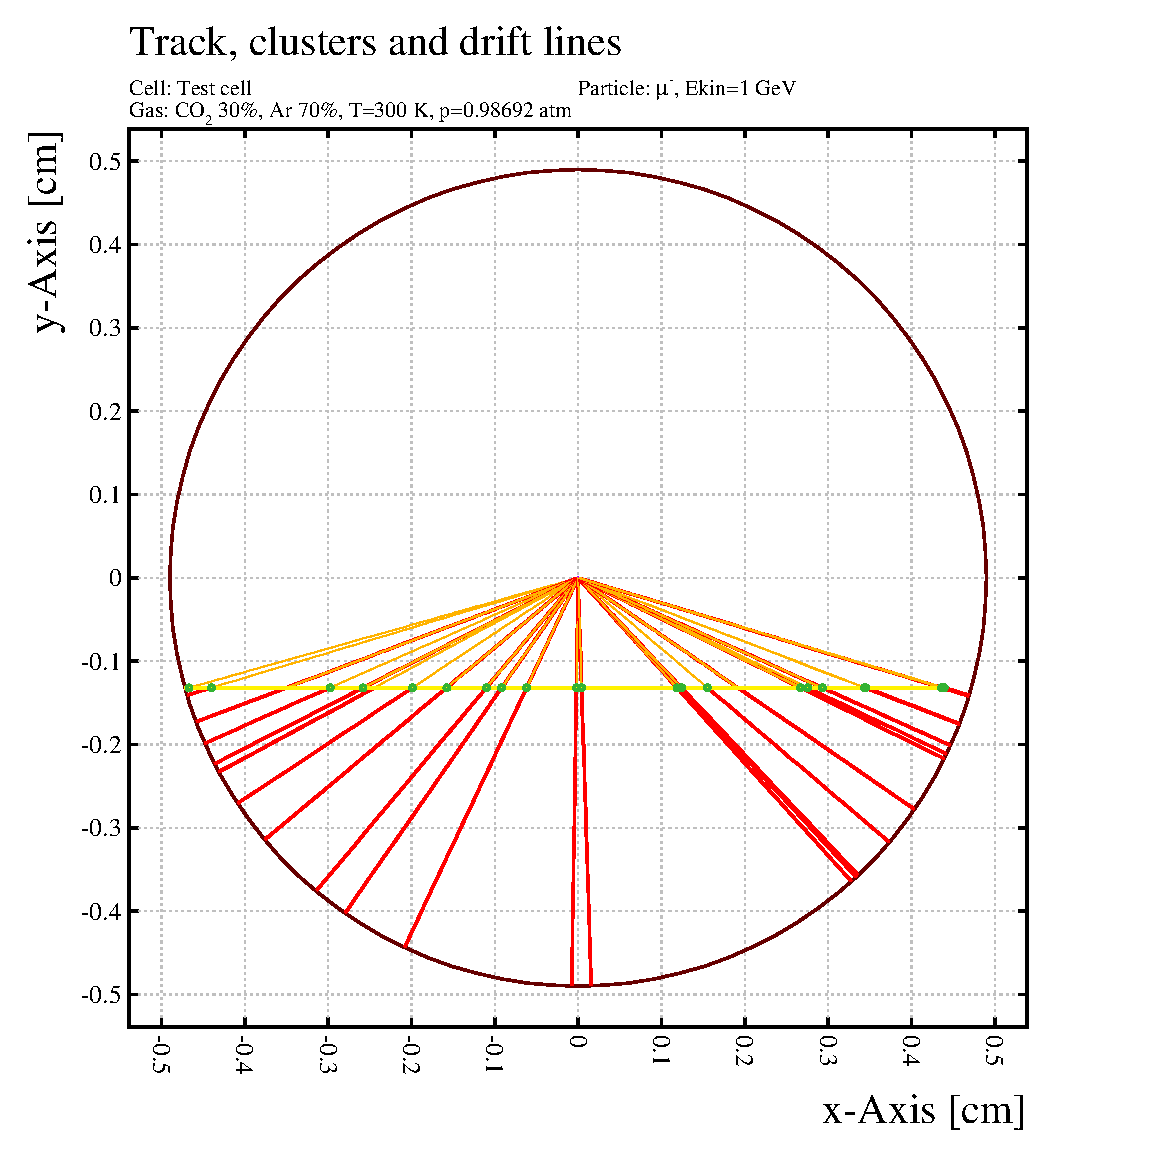
\includegraphics[width=0.43\textwidth]{sag/tracksAndClusters00Sag.eps} 
			\label{fig:electron_ion_track} }%
		\qquad
		\subfloat[дріс зміщений від центру трубки на 1.4мм]{
			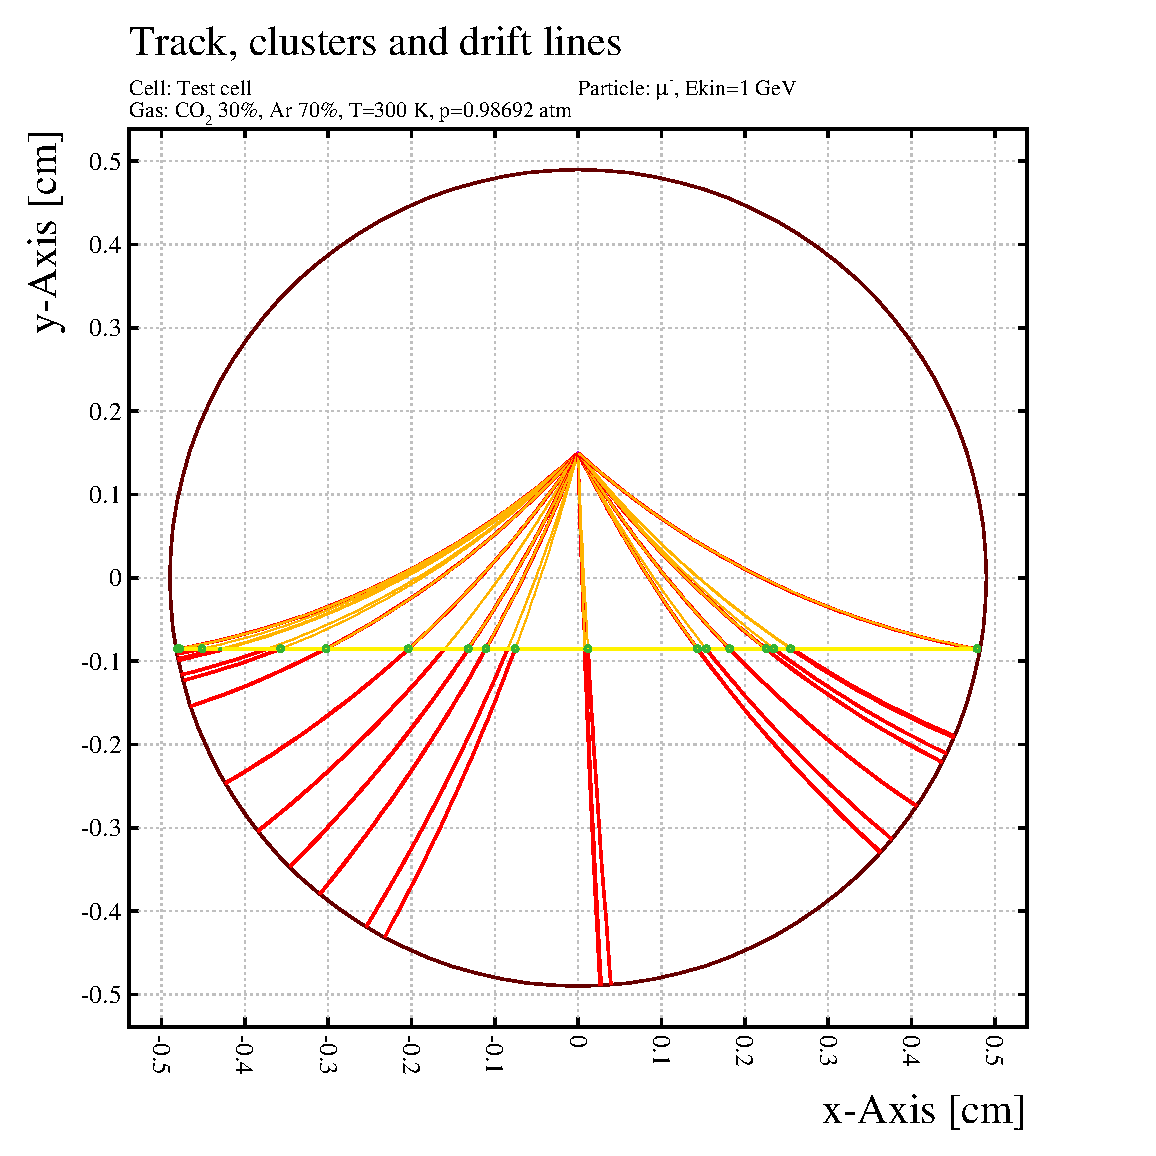
\includegraphics[width=0.43\textwidth]{sag/tracksAndClusters15Sag.eps} 
			\label{fig:electron_ion_track_sag} }%
		\caption{ Приклад траєкторій треків іонів і електронів в трубці для різних положень дроту. Рисунки є симуляціями і експортувалися безпосередньо з середовища GARFIELD. Місця утворення початкових кластерів позначено зеленим кольором. Лінії дрейфу електронів позначено жовтим кольором, іонів - червоним.}
%		\caption{ An example of tracks from the on the tube for different position of the wire from GARFIELD simulations. Initial clusters marker by green. Drift lines for electrons marked by yellow, ions -- red lines.}	
	\end{figure}
	
	Напрям провисання провисання дроту для дрейфової трубки розташованої вертикально неможливо, так як фактор гравітації тут не грає ролі. Проте в горизонтальному положенні такої неоднозначності нема. Від так, умова горизонтального положення дрейфових трубок горизонтально є необхідною для можливості знаходити положення треків у трубці з високою точністю і з допуском провисання дроту (положення дроту в середині нічим не фіксується).
	
	Навіть сильно натягнуті дроти з силою $T$ близькою до межі міцності довжиною в декілька метрів будуть значно провисати під дією гравітаційного поля. І провисання буде досягати значень значно більших за точність реконструкції треків, яку можна досягнути за допомогою дрейфової трубки.
	
%	The direction of sagging is unpredictable when the wire is centered and the straw has vertical orientation. Impact of gravitation field into the wire does not make any effect in this state. But we can avoid this ambiguity by setting straws horizontally. This condition is necessary to make track reconstruction possible.
%	Even when strung with a pulling force $T$ close to the breaking limit, wires in several metre long tubes will experience a gravitational sag that is large in comparison with the achievable accuracy of drift tubes.
	
	Очікується значне провисання дроту(порівняно навіть до радіусу трубки) так як поряд  з гравітаційним полем присутнє ще й електричне поле.
	
%	We estimate significant wire sagging(by comparison to the tube radius) because of wire attracts to the tube under affecting of gravitation and electric field force.

	Профіль провисання дроту довжиною $5m$ в трубці діаметром 1см і напругою 1750В показано на Рис.\ref{fig:sagProfile} розрахований в програмному пакеті GARFIELD \cite{garfield}.
		
%	You can see a profile of wire sagging of $5m$ length wire in $1cm$ diameter straw tube and 1750V voltage on the fig.\ref{fig:sagProfile} calculated in GARFIELD software \cite{garfield}.
	
	\begin{figure}[h!]
	\centering
	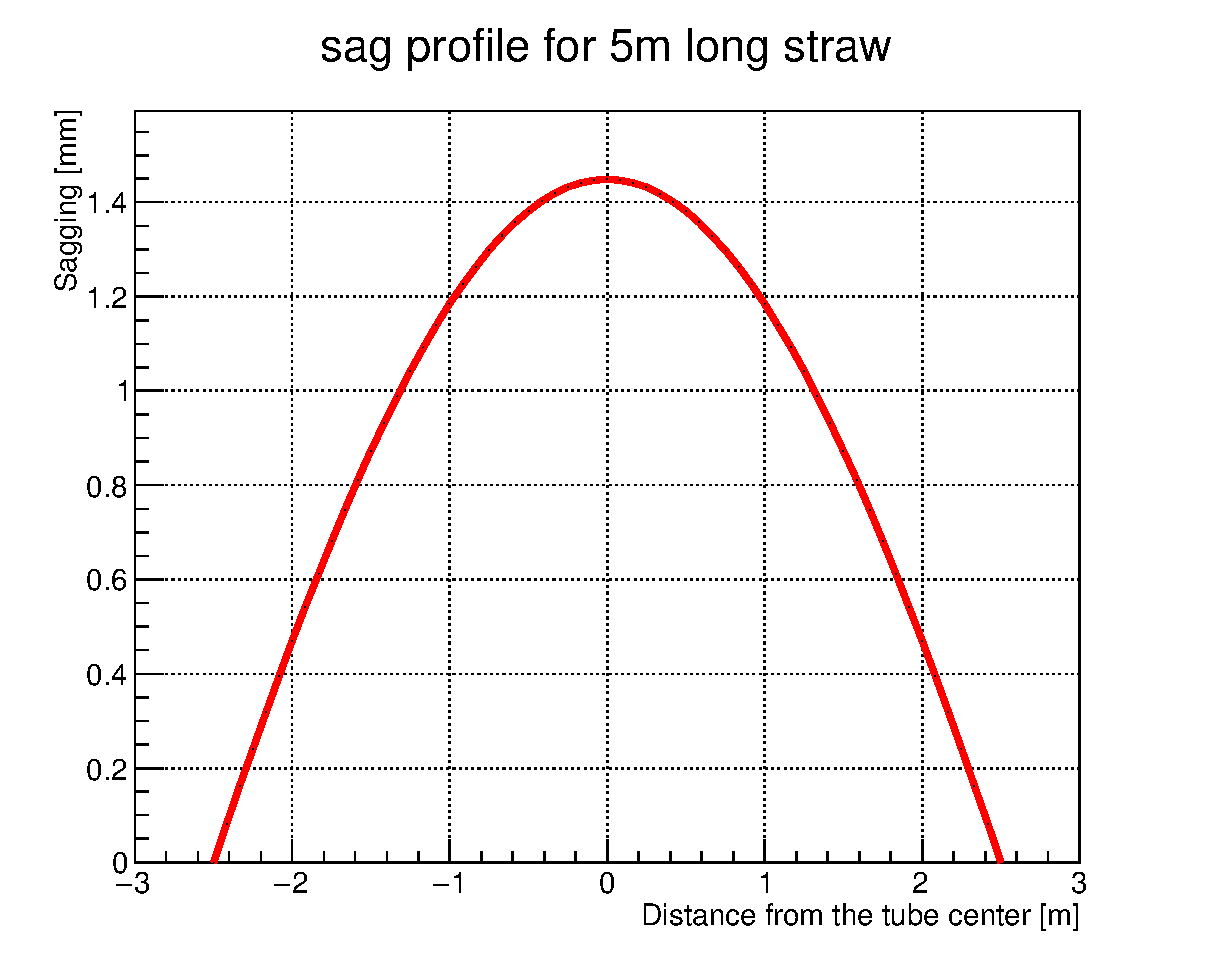
\includegraphics[width=0.7\textwidth]{sagProfileFit.eps}
	\caption{Профіль провисання дроту під дією гравітаційного та електричного полів розраховаий в програмному пакеті GARFIELD.}
%	\caption{Wire sag profile under electric and gravitation field calculated in GARFIELD. All options for this straw system are described in table~\ref{table:straw_par}.}
	\label{fig:sagProfile}
	\end{figure}	
	
	Калібровка дрейфової трубки з провиснутим дротом є більш складною порівняно до дизайну де положення дроту фіксовано по центру.
%	The calibration of STRAW tube with sagged wire is more difficult by comparison to the mode without sagging. 

	Варіація сили розтягу дроту, радіус дроту розглядаються як параметри, які можливо змінити при виробництві. І вони можуть змінюватися для підбору оптимальних значень необхідних для ефективної роботи трубки.
		
%	Variation of wire tension, wire radius should be taken into account as high affect factor for sag value.
	
	\section{ Оцінка провисання трубки}

	В цьому розділі ми маємо знайти метод, що дозволяв би вимірювати зміщення дроту. Це ключовий крок до можливості реконструкції треків.
%	In this section we have to find out method for assessing sagging. This is key step that makes track reconstruction procedure possible.

	Для	початку необхідно подумати над даними які нам можуть бути доступними для досягнення цієї цілі. В даному випадку найбільш привабливим є розподіл треків по часу дрейфу.
%	At first we have to think on data we can use for such kind of calculations. Much attractable information we can extract from drift time distribution. 

	Дріт провисає під дією електричного і гравітаційного поля. Таким чином значення зміщення дроту  від центрального положення змінюється вздовж трубки(див. Рис.\ref{fig:sagProfile}). Але очевидно в умовах використання дрейфових трубок знайдеться спосіб хоча б грубо розділити дані для різних частин трубки( хоча б з міркувань перехресності шарів дрейфових трубок). Тож при необхідності повздовжній параметр треку розрізнити можна. В лабораторних умовах для цих цілей можна використовувати й інші детектори.
	
%	The wire sags under electric and gravitation force. Therefore the sag value is differ along the tube(fig~\ref{fig:sagProfile}). But we can separate collected data for different position along the tube. STRAW tube detector consist of several parallel layers of tubes at some angle to each other. So we can easily fix longitudinal position(along the tube)  for tracks that cross several crossed tubes(at least two). Collimation is also possible via scintillator triggering before and after STRAW tube.

	Нехай ми помістили дрейфову трубку в однорідний потік  мюонів і зберегли гістограму розподілу треків за часом дрейфу для певної позиції дроту. Як було досліджено за допомогою пакету GARFIELD такі розподіли відрізняються для кожного значення зміщення дроту(Див. приклад на Рис.\ref{fig:DrftTimeDistr_00_09_comp}). Різниця в розподілах тим більша чи більша відносна різниця в між значеннями зміщення дроту для першої і другої діаграми.
%	Lets say we can install our STRAW tube into homogeneous particle flow and save drift time distribution for some narrow section of the tube. These distributions are different from each other(see example on Fig.\ref{fig:DrftTimeDistr_00_09_comp}). The difference between diagrams increasing with sag difference. So it is good tools for sag calibration.
		
	\begin{figure}[h!]
	\centering
	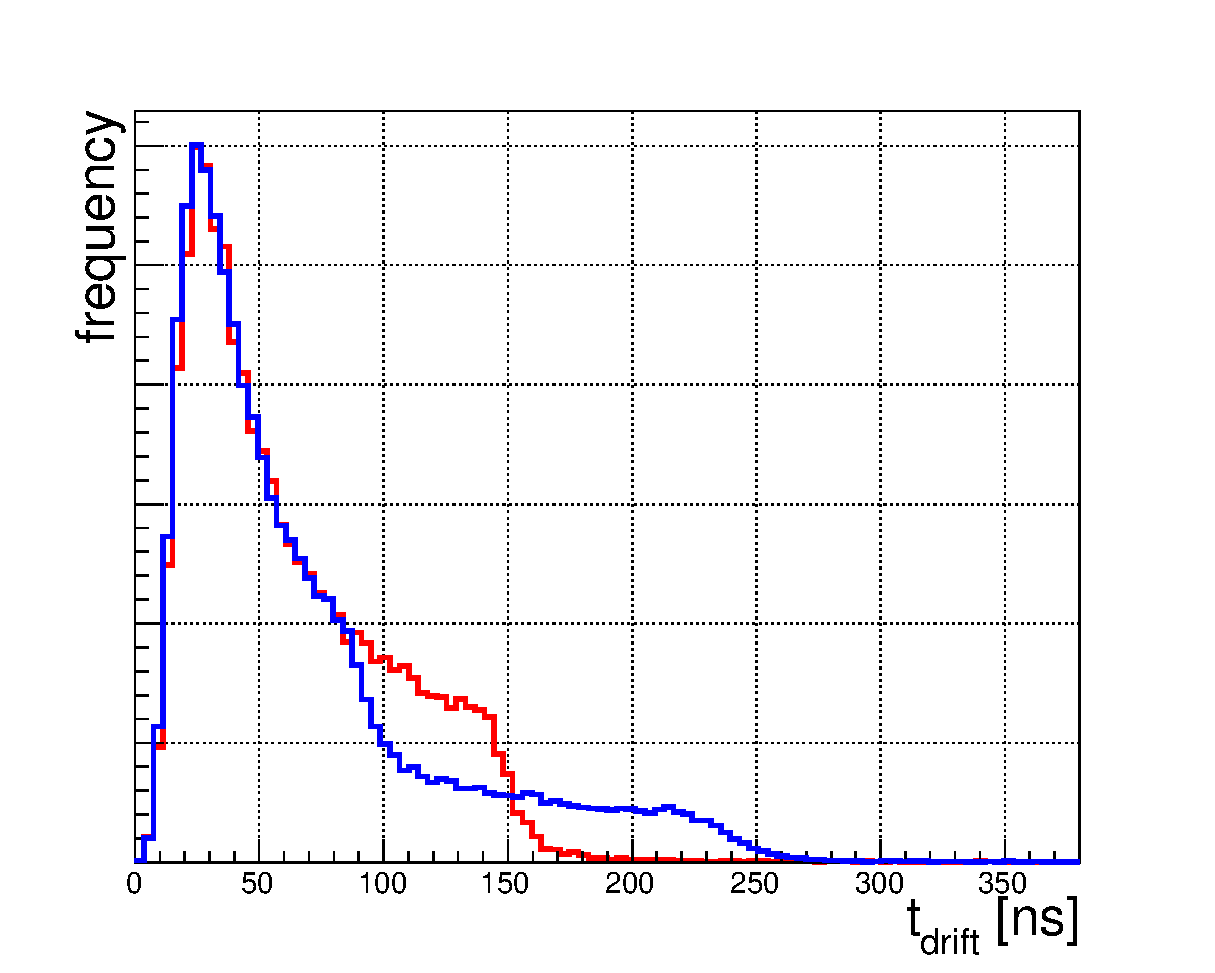
\includegraphics[width=0.8\textwidth]{00_09_driftTimeDistr}
	\caption{ Розподіл часу дрейфу від однорідного потоку мюонів для двох значень позиціх треків: для центрованого дроту (червона гісограма) і для випадку зміщення дроту на 0.9 мм відносно центру (синя гістограма).}
%	\caption{Drift time distribution for a homogeneous irradiation with a centered wire (red) and for a wire offset of 0.9 mm (blue).}
	\label{fig:DrftTimeDistr_00_09_comp}	
	\end{figure}

	Потім необхідно пов’язати окрему форму розподілу часу дрейфу з відповідним значення провисання дроту. Це частина роботи лабораторного перед експериментального етапу. Вимірювання профілю провисання дроту може бути виконано оптичним методом, оскільки стінки дрейфової трубки дуже тонкі, звичайним просвіченням об'єму трубки збоку.	
%	Then we have to bind each drift time distribution with appropriate sag value. This is part of laboratory work when sag profile measurements can be performed via optical method prior to the exposition.
	
	Розподіли на Рис.\ref{fig:DrftTimeDistr_00_09_comp} містять GARFIELD симуляції для певних точних значень положення дроту (не для певної секції). Це дуже важливо і буде особливістю даних змодельованих в GARFIELD і отриманих на експерименті. 
%	Distributions on graph~\ref{fig:DrftTimeDistr_00_09_comp} contain GARFIELD simulations for some certain wire(not for section of sagged wire)because of GARFIELD can handle only two-dimensional tasks.

	Нехай ми маємо приладдя для сканування профілю трубки. Після виміру профілю ми розділяємо трубку на віртуальні секції, достатньо вузькі для того, щоб точність визначення позиції дроту і кількість секцій були в  розумних межах. Вважаємо положення дроту в межах однієї секції сталим.
	
%	Lets say we have an equipment for scanning the tube to measure wire sagging profile. After profile measurements we divide our tube into sections. Wire position within separate section should be within desired precision.
	
	Для досягнення точності визначення позиції дроту  в $50\mu m$ грубим методом(дивись наступний розділ) в трубці необхідно виділити 57 частин.
%	So we need divide our tube into $57$ sections (see figure~\ref{fig:tube_sectioning}) if maximum of wire offset(at the center of the tube) is equal to $1.45mm$ and desired precision is $50\mu m$.
	
	\begin{equation}
	N_{halftube} = \frac{1.45 mm}{50 \mu m} = 29;
	\label{eq:tube_sectioning}
	\end{equation}
	
	\begin{figure}[h!]
	\centering
	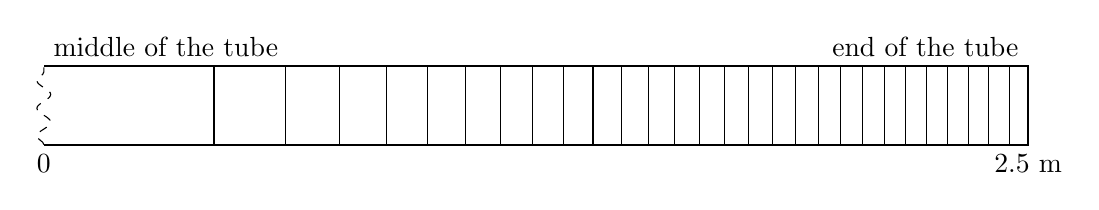
\begin{tikzpicture}[xscale=0.05,yscale=1]
	
	\tikzset{snake it/.style={decorate, decoration=snake}}
	\draw[snake it,dashed] (0,0) -- (0,1);
	
	\draw[thick] (0,0) -- (250,0) -- (250,1) -- (0,1);
	\draw[] (43.2339,0) -- (43.2339,1) -- 
	(61.2704,1) -- (61.2704,0) -- 
	(75.2004,0) -- (75.2004,1) -- 
	(87.0213,1) -- (87.0213,0) -- 
	(97.5056,0) -- (97.5056,1) -- 
	(107.049,1) -- (107.049,0) -- 
	(115.885,0) -- (115.885,1) -- 
	(115.885,1) -- (115.885,0) -- 
	(124.169,0) -- (124.169,1) -- 
	(132.005,1) -- (132.005,0) -- 
	(139.472,0) -- (139.472,1) -- 
	(146.627,1) -- (146.627,0) -- 
	(153.516,0) -- (153.516,1) -- 
	(160.176,1) -- (160.176,0) -- 
	(166.636,0) -- (166.636,1) -- 
	(172.921,1) -- (172.921,0) -- 
	(179.05,0) -- (179.05,1) -- 
	(185.043,1) -- (185.043,0) -- 
	(190.913,0) -- (190.913,1) -- 
	(196.674,1) -- (196.674,0) -- 
	(202.338,0) -- (202.338,1) -- 
	(207.915,1) -- (207.915,0) -- 
	(213.414,0) -- (213.414,1) -- 
	(218.844,1) -- (218.844,0) -- 
	(224.212,0) -- (224.212,1) -- 
	(229.527,1) -- (229.527,0) -- 
	(234.793,0) -- (234.793,1) -- 
	(240.018,1) -- (240.018,0) -- 
	(245.207,0) -- (245.207,1);
	
	\node[below] at (0,0) {0};
	\node[below] at (250,0) {2.5 m};
	\node[above right] at (0,1) {middle of the tube};
	\node[above left] at (250,1) {end of the tube};
	
	\end{tikzpicture} 
	\caption{ Секціонування трубки по довжині. Максимальне значення зміщення дроту знаходиться по цетру і рівна 1.45 мм. Різниця між секціями для величини зміщення становить $50\mu m$ }
%	\caption{Tube sectioning. Sag value at the tube center is $1.45mm$. Difference of wire sag value from section to section is $50\mu m$}
	\label{fig:tube_sectioning}
	\end{figure}
	
	Для отримання точних результатів аналізу розподіл часу дрейфу нам необхідно мати якомога вищу статистику(на цей час достатньою статистикою можна вважати 50 тис подій). Слід зазначити, що для досягнення такої статистики секціям на периферії знадобиться значно більше часу як для центральних секцій.
	
%	Then we need an exposition of sufficient number of events for every of sections(at least 50k events). There can be troubles time of exposition time because square of sections at the end of the tube is quite small. So the time of exposition of distant sections will be inversely much longer.
	
%	The next step is to find dependence of dt-distribution shape with wire offset. The point that we can evaluate matching between histograms via $\chi^2$  criteria. As we can see in the figure~\ref{fig:chi2for07} the comparison of  $\chi^2$ has smooth dependence across increasing of wire offset for high statistic histograms.

	Кроки, необхідні для вимірювання позиції дроту:
%	First steps for sag estimation are:
	\begin{enumerate}
	\item виміряти профіль дроту оптичним методом;
	\item cекціонувати трубку;
	\item опромінити і записати розподіли часу дрейфу з гарною статистикою. Такі гістограми будемо називати базовими, і в наступних кроках будемо їх використовувати в ролі еталонних.
	\item Для знаходження позиції дроту шляхом самого порівняння необхідно знайти розподіл часу дрейфу для шуканого відрізку і порівняти з усіма базовими розподілами(гістограмами).
	\item Найкраща відповідність дасть найбільш правдоподібне значення зміщення дроту
%	\item measure wire sag profile via optical method;	
%	\item make a sectioning for wire sag profile;
%	\item collect enough amount of events for every of dt-distribution and save this {\it core} distribution for further comparisons.
%	\item measure dt-distribution for new drift tube section that is subject of study.
%	\item calculate $\chi^2$ criteria for this current dt-distribution with each of core distribution. 
	\end{enumerate}

	\subsection{ Знаходження найбільш правдоподібного положення дроту в трубці}
	
	\subsection{Грубий метод}
	
	Найпростіший метод для знаходження положення дроту $S$ полягає в тому, щоб вважати найбільш імовірним значення відхилення дроту  $S$ те, для розподілу якого  число схожості(аналог $\chi^2$) DT-розподілів найменше .
%	The simplest method to find $S$ is to equate it to the corresponding value of best matched core DT-histogram.

	На рисунку 	\ref{fig:chi_063_5k} зображено розподіл для $S$ від знайдених по вищеописаному методу. В даному випадку статистика DT-розподілів сягала всього 5 тисяч. Як можна бачити точність такого методу рівна числу дискретизації контрольних діаграм які розташовані на відстані 50 мікрометрів одна від одної.
%	On the figure \ref{fig:chi_063_5k}  you can see distribution of such kind of reconstruction. Even for 5k events td-distribution in this case the precision can be quite high($\sim 50 \mu m$). This method limited by core DT-diagram stepping.
	
	До недоліків грубого методу можна віднести необхідність частої дискретизації базових DT-розподілів.
	\begin{figure}[h!]
		\centering
		\subfloat[Серія $\chi^2$ порівнянь гістограми для $S = 0.7 mm$ з кожною із базових діагнам.]{
			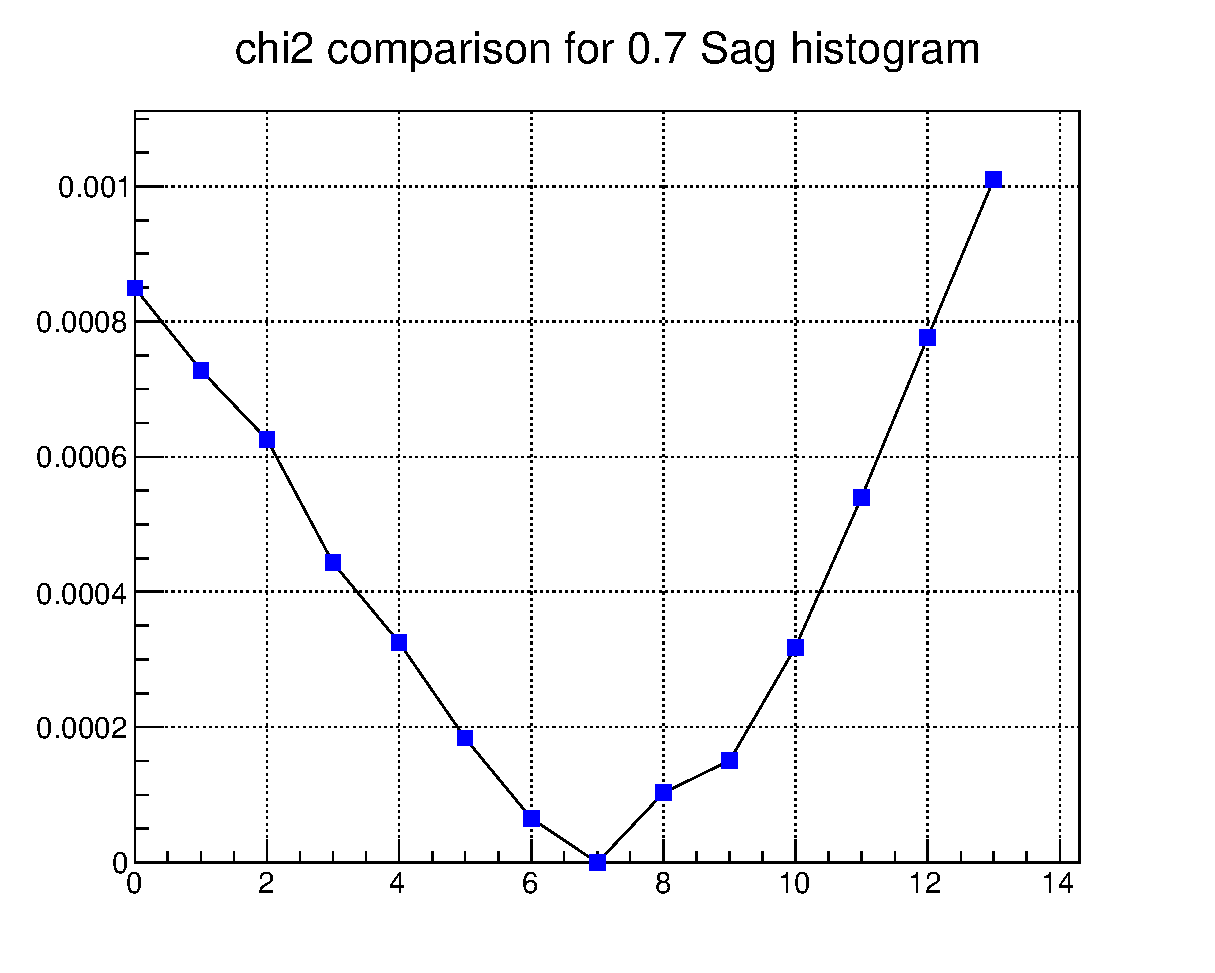
\includegraphics[width=0.43\textwidth]{chi2_07} 
			\label{fig:chi2for07} }%
		\qquad
		\subfloat[ Розподіл реконструйованих значень відхилення дроту від центрального положення від 180 серій порівнянь для 5 тис. гістограм з  50 тисячними базовими гістограмами. Реальне значення положення дроту для всіх 5 тис. гістограм  становить $0.63 mm$.]{
			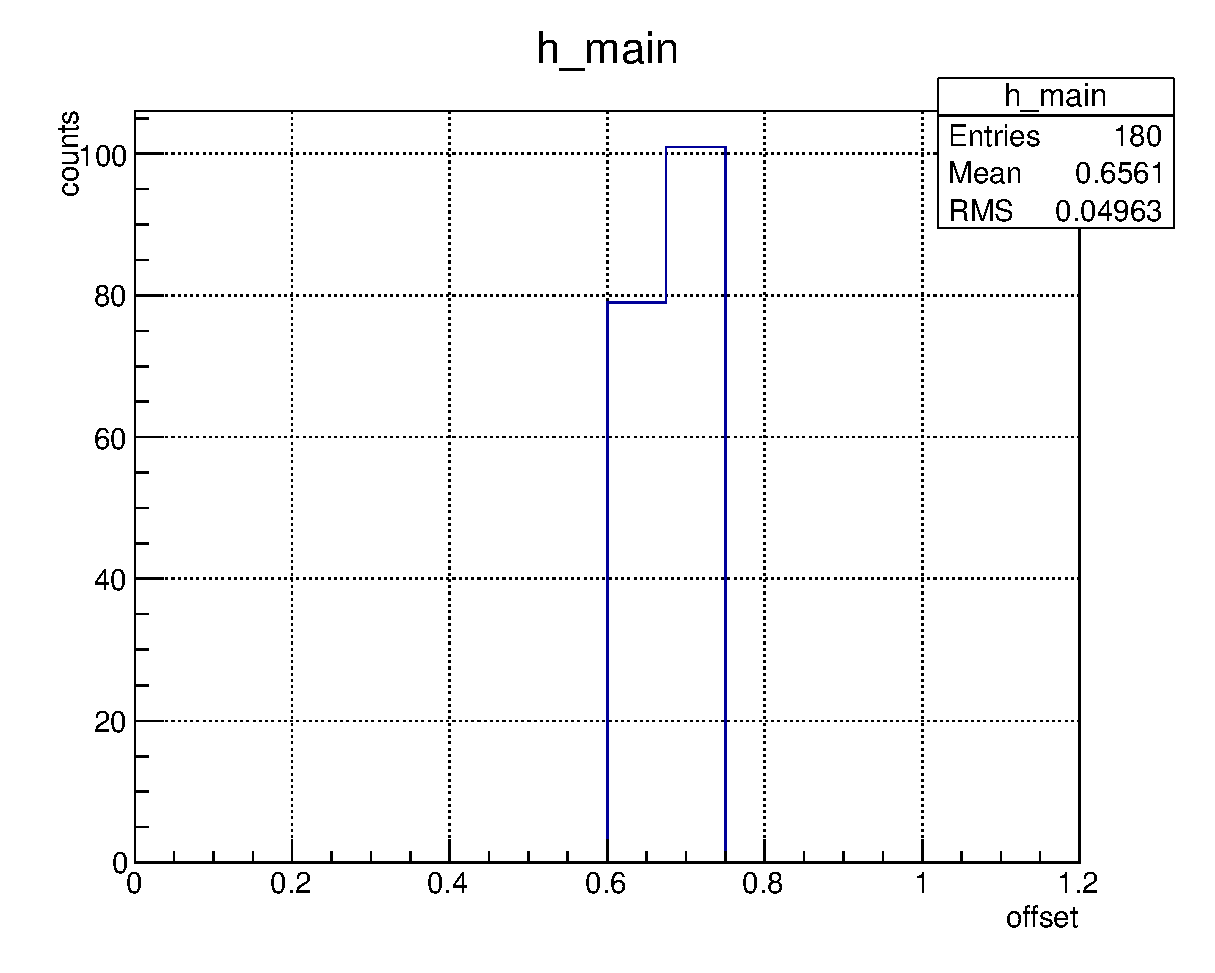
\includegraphics[width=0.43\textwidth]{chi_063_5k} 
			\label{fig:chi_063_5k} }%
		\caption{Реконструкція положення дроту}			
	\end{figure}	
	
%	If we compare dt-distribution for $0.7mm$ displaced wire with each of core dt-distribution you will notice best matching with core histogram for the same wire displacement(see fig see fig~\ref{fig:chi2for07}).
	
\begin{comment}
	\subsection{Minimum of $\chi^2$ as linear approximation}
	But what is most probable value of wire displacement $S$ in this case? Probably somewhere between them. So can we go in more clever way to reach better result? Probably yes.
	
	If dependence of $\chi^2$ criteria of wire displacement $S$ for near to the true position region is linear(that certainly is not a true, but as first approximation) than we can easily find this intermediate value of wire displacement.
	
	There we proceed in two steps. The first is raw estimation of wire displacement as in above mentioned method.
	
	For the second step we need to know some additional estimations.	The first question is how small can be  $\chi^2$ it our case? Lets fix statistic on 50k events for one DT-distribution. This value should a bit depend for different $S$. But for now lets consider that it is a constant value. From the figure \ref{fig:chi2Shelf} you can see distribution of $\chi^2$ from comparison of 20 DT-distribution\footnote{pair comparison give us $C_{20}^2 = \frac{20!}{2!18!}=190$ different combinations}  for $S=0.7mm$. Mean value + RMS of distribution is $ 5.3*10^{-5}$. So if some of the $\chi^2$ is higher than this threshold than we go for second stage.
	
	
	\begin{figure}[h!]
		\centering
		\subfloat[$\chi^2$ distribution of comparison of 20 DT-distributions diagrams each other($C_{20}^2 = 190$ combinations)]{
			\includegraphics[width=0.43\textwidth]{chi2Shelf} 
			\label{fig:chi2Shelf} }%
		\qquad
		\subfloat[$\chi^2$ distribution of comparison DT-distribution histograms $0.6 mm$ S vs $0.7 mm$ ]{
			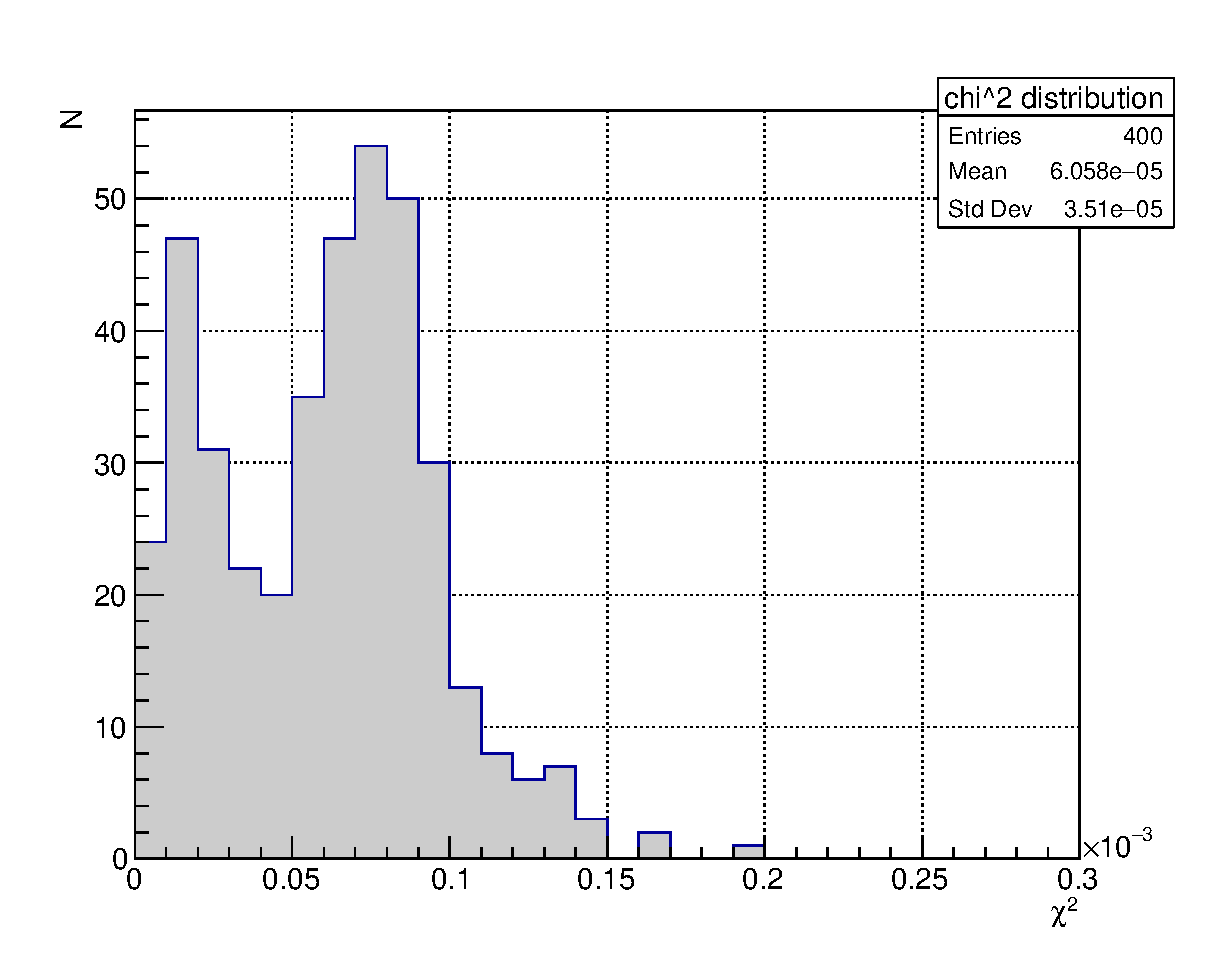
\includegraphics[width=0.43\textwidth]{06_07_chi_stat} 
			\label{fig:06_07_chi_stat} }%
		\caption{Comparison of $\chi^2$ distributions for self-comparison of DT-distribution diagram.} 
	\end{figure}	
	
	On the figure \ref{fig:chi_063_5k} you can see distribution wire sag calculation for 180 histograms with 5k events statistic. Precision in this case  $\sim 50\mu$. The algorithm of sag estimation is pretty simple: wire offset value eual to the as best match between $test$ and $core$ histogram.

	After we know sag value at some points of the tube or every where we can make one awesome collective analysis. The smoothing of wire offset value along the tube will give us much more precision results.  
	
	From the Fig.\ref{fig:06_07_chi_stat} the distribution of $\chi^2$ for adjasent point have narrower distribution by comparison to "self-comparison" $\chi^2$ distribution. Therefore method of reconstructing of wire offset that based on comparison of DT-distribution histogram can find  wire offset much precisely.
	
	
\end{comment}	
	
	\subsection{ Cхема реалізації сепарації треків}
	
	В даному випадку нам потрібно мати додатковий позиційно чутливий детектор, що реєстрував би мюон. Це може бути будь’який детектор, починаючи від газового до сцинтиляційного.
	
%	We need second detector that can measure position of muon that hit STRAW tube. It can be Si strip sensor based detector or detector based on  scintillation with the same destination.

	Кожен з детекторів має свої переваги та недоліки. Так силіконові полоскові детектори можуть забезпечити чудову точність, проте покрити всі 5м дрейфової трубки буде складно і дорого. Найкращим на мою думку тут є використання сцинтиляційних елементів достатньо великого розміру(порядку найменших секторів трубки.
%	Each kind of detector have it's own advantages and disadvantages. The potential cell unit (strip of pixel) of Si detector will be smaller than in scintilator but also is match expensive. At the current stage we deal with $1cm$ diameter tubes. So scintilator is primal target. But it can shift to the Si sensors if scintilators will not provide satisfied precision.

	Попередня схема постановки експерименту з експозиції і сепарації треків з вимірювання DT-розподілу.	
%	Preliminary chem of DT-measurements you can see on the picture Fig.\ref{fig:DT-mesure-layout}
	
	\begin{figure}[h!]
	\centering
	\begin{tikzpicture}
	
	\tikzset{snake it/.style={decorate, decoration=snake}}
	
	\draw (-1,0) -- (-1,10);
	\draw ( 1,0) -- ( 1,10);
	\draw (0,0) ellipse (1 and .3);
	\draw (0,10) ellipse (1 and .3);
	
	\draw (-5,0) -- (-6,0);
	\draw (-5,.5) -- (-6,.5);
	\draw (-5,1) -- (-6,1);
	\draw (-5,1.5) -- (-6,1.5);
	\draw (-5,2) -- (-6,2);
	\draw (-5,2.5) -- (-6,2.5);
	\draw (-5,3) -- (-6,3);
	\draw (-5,3.5) -- (-6,3.5);
	\draw (-5,4) -- (-6,4);
	\draw (-5,4.5) -- (-6,4.5);
	\draw (-5,5) -- (-6,5);
	\draw (-5,5.5) -- (-6,5.5);
	\draw (-5,6) -- (-6,6);
	\draw (-5,6.5) -- (-6,6.5);
	\draw (-5,7) -- (-6,7);
	\draw (-5,7.5) -- (-6,7.5);
	\draw (-5,8) -- (-6,8);
	\draw (-5,8.5) -- (-6,8.5);
	\draw (-5,9) -- (-6,9);
	\draw (-5,9.5) -- (-6,9.5);
	\draw (-5,10) -- (-6,10);
	
	\draw (-5,0) -- (-5,10);
	\draw (-6,0) -- (-6,10);

	\draw (5,0) -- (6,0);
	\draw (5,.5) -- (6,.5);
	\draw (5,1) -- (6,1);
	\draw (5,1.5) -- (6,1.5);
	\draw (5,2) -- (6,2);
	\draw (5,2.5) -- (6,2.5);
	\draw (5,3) -- (6,3);
	\draw (5,3.5) -- (6,3.5);
	\draw (5,4) -- (6,4);
	\draw (5,4.5) -- (6,4.5);
	\draw (5,5) -- (6,5);
	\draw (5,5.5) -- (6,5.5);
	\draw (5,6) -- (6,6);
	\draw (5,6.5) -- (6,6.5);
	\draw (5,7) -- (6,7);
	\draw (5,7.5) -- (6,7.5);
	\draw (5,8) -- (6,8);
	\draw (5,8.5) -- (6,8.5);
	\draw (5,9) -- (6,9);
	\draw (5,9.5) -- (6,9.5);
	\draw (5,10) -- (6,10);
	
	\draw (5,0) -- (5,10);
	\draw (6,0) -- (6,10);
	
	\node [below] at (5,0) {detector 2};
	\node [below] at (-5,0) {detector 1};
	\node [] at (0,-1) {STRAW tube};


	\draw[ultra thick,->] (-10,7.5) -- (-6.5,7.5);
	\draw[ultra thick,->] (-10,7) -- (-6.5,7);
	\draw[ultra thick,->] (-10,6.5) -- (-6.5,6.5);
	\draw[ultra thick,->] (-10,6) -- (-6.5,6);
	\draw[ultra thick,->] (-10,5.5) -- (-6.5,5.5);
	\draw[ultra thick,->] (-10,5) -- (-6.5,5);
	
	\node at (-8,8) {muon flow};
	
	\draw[thick] (-8,3) ellipse (0.3 and 0.3);
	
	\draw[thick] (-8-0.2, 3-0.2) --(-8 +0.2, 3+0.2);
	\draw[thick] (-8-0.2, 3+0.2) --(-8 +0.2, 3-0.2);

	\node[] at (-8.5,3) {$\vec{g}$};
		
	\end{tikzpicture} 
	\caption{схема постановки експерименту з експозиції і сепарації треків для вимірювання DT-розподілу}
%	\caption{principal layout of measurement of core DT-distribution histogram}
	\label{fig:DT-mesure-layout}
	\end{figure}	
	
	Головна вимога для даної установки - забезпечити достатню точність для сепарації треків по блокам дрейфової трубки. Приклад секціонування трубки зображено на Рис.\ref{fig:tube_sectioning}. Також детектори D1 та D2 мають забезпечувати достатній асептанс. Потік мюонів повинен бути рівномірним --це обов’язкова умова для даної задачі також.

	Справжній же профіль може бути виміряний оптичним методом, так як стінки трубки дуже тонкі.
%	In this method detector before tube (D1) and detector placed after the tube(D2) in total should provide sufficient precision for track reconstruction to be able distinguish tracks for different section of the tube (approximately as shown on the Fig. \ref{fig:tube_sectioning}). Muon flow should be homogeneous and so D1 and D2 also should cover full acceptance of the tube.
	
%	The profile of wire sagging can be measured by optical method. Wall of is very thin, so it can be simplest way to get sag profile.
	